%% Fig. 1 of the article: overview of the planner with the learned examination order (schematic, no data).
%% Built at the column width of the template (76 mm), Helvetica 8 pt.
\documentclass[border=0.5pt]{standalone}
\usepackage[T1]{fontenc}
\usepackage{textcomp}
\usepackage{helvet}
\renewcommand{\familydefault}{\sfdefault}
\usepackage{tikz}
\usetikzlibrary{positioning,arrows.meta,fit,calc}
\definecolor{learned}{RGB}{0,114,178}
\definecolor{orig}{RGB}{90,90,90}
\begin{document}
\fontsize{8}{9.4}\selectfont
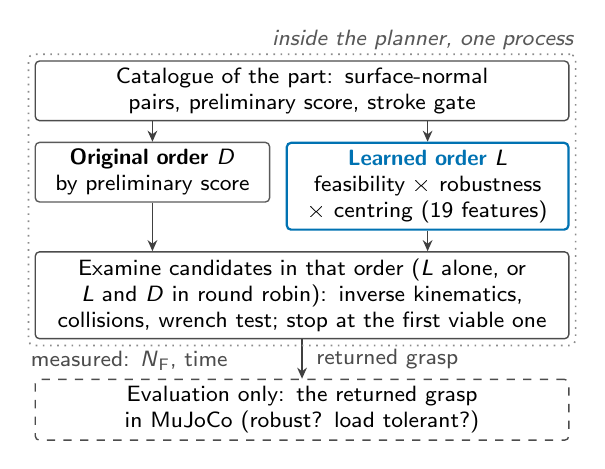
\begin{tikzpicture}[
    box/.style={draw=black!70, rounded corners=1.5pt, align=center, inner sep=2.5pt, line width=0.5pt,
      font=\fontsize{8}{9.4}\selectfont},
    arr/.style={-{Stealth[length=4pt,width=3.5pt]}, line width=0.6pt, black!75},
    node distance=2.6mm]
  \node[box, text width=66mm] (cat) {Catalogue of the part: surface-normal pairs, preliminary score, stroke gate};
  \node[box, text width=28mm, below=of cat.south west, anchor=north west, draw=orig] (orig)
    {\textbf{Original order} \textit{D}\\by preliminary score};
  \node[box, text width=34mm, below=of cat.south east, anchor=north east, draw=learned, line width=0.8pt] (learn)
    {\textbf{\color{learned}Learned order} \textit{L}\\feasibility \texttimes{} robustness\\\texttimes{} centring (19 features)};
  \path (learn.south) ++(0,-2.6mm) coordinate (eb);
  \node[box, text width=66mm, anchor=north] (exam) at (cat.south |- eb)
    {Examine candidates in that order (\textit{L} alone, or \textit{L} and \textit{D} in round robin):
     inverse kinematics, collisions, wrench test; stop at the first viable one};
  \node[box, text width=66mm, below=5mm of exam, dashed] (sim)
    {Evaluation only: the returned grasp in MuJoCo (robust? load tolerant?)};
  \draw[arr] (cat.south -| orig.north) -- (orig.north);
  \draw[arr] (cat.south -| learn.north) -- (learn.north);
  \draw[arr] (orig.south) -- (orig.south |- exam.north);
  \draw[arr] (learn.south) -- (learn.south |- exam.north);
  \draw[arr] (exam) -- node[right=1.5pt, font=\fontsize{8}{9}\selectfont, text=black!70] {returned grasp} (sim);
  \node[draw=black!45, dotted, line width=0.6pt, rounded corners=2pt, inner sep=2.2pt, fit=(cat)(orig)(learn)(exam)] (planner) {};
  \node[anchor=south east, inner sep=1pt, font=\fontsize{8}{9}\selectfont\itshape, text=black!65]
    at (planner.north east) {inside the planner, one process};
  \node[anchor=north west, inner sep=1pt, font=\fontsize{8}{9}\selectfont, text=black!70]
    at ([yshift=-0.5pt]planner.south west) {measured: \textit{N}\textsubscript{F}, time};
\end{tikzpicture}
\end{document}
